\documentclass[../sparc.tex]{subfiles}
\graphicspath{{\subfix{../images/}}}
\begin{document}

%%%%%%%%%%%%%%%%%%%%%%%%%%%%%%%%%%%%%%%%%%%%%%%%%%%%%%%%%%%%%%%%%%%%%%%%%%%%%%%%
\section{I2C bus}
\label{section:i2c}
\index{Electronics!I2C bus}

\newglossaryentry{I2C}{
  name=I2C,
  description={Inter-Integrated Circuit}
}
\newglossaryentry{USB}{
  name=USB,
  description={Universal Serial Bus}
}
\newglossaryentry{PCI}{
  name=PCI,
  description={Peripheral component interconnect}
}
\newglossaryentry{I/O}{
  name=I/O,
  description={I/O -- ``Input/Output''}
}

%%%%%%%%%%%%%%%%%%%%%%%%%%%%%%%%%%%%%%%%%%%%%%%%%%%%%%%%%%%%%%%%%%%%%%%%%%%%%%%%
\subsection{General information}

\textit{\gls{I2C}} also sometimes called $I^{2}C$ (should be read as
``I-squared-C'') is a data transfer bus that is used for connection between
integrated circuits inside electronic devices.  Let's discuss first what a
``data bus'' is.  To put it simply a \textit{bus} in the context of the computer
architecture is some connection that is used for data transferring between
functional parts of a computer.

We can put data transfer buses roughly into two categories -- \textit{external}
buses and \textit{internal} buses.

External buses include \gls{USB} which is already familiar for many of us -- this
bus is used for connection of external devices (such as Arduino, a keyboard, a
computer mouse, a printer and so on) to a computer.  Such buses usually have
some standardized connector and fairly big length of the cable.

Internal buses include \gls{I2C} (already mentioned above) and \gls{PCI}/PCI
Express (used for example for connection of a network card to the computer
system board.)  Internal buses are usually designed for transferring data across
short distances, and don't allow hot-plugging of devices; thus some of the
internal buses don't even have a special connector and bus wires are soldered
down right to the boards.

The maximum length of connection between devices on \gls{I2C} bus should not
exceed 30 centimeters, otherwise data transfer will be unreliable.

\gls{I2C} has quite low data transfer speed (no more than 5MBit/s) between
devices.  Each device has its own \textit{address} on the bus -- in other words,
its serial number.  We can connect up to 127 devices with unique addresses.
With that said, we must note that only one device on the bus is the controller
while the rest of the devices are targets.

On the fig. \ref{fig:i2c-schematics} the \gls{I2C} bus schematic is shown.  As
we can see on the figure, the bus uses only two lines for data transferring --
``Serial Data Line'' (\textbf{SDL}) and ``Serial Clock Line'' (\textbf{SCL}.)
Both lines are pulled up through resistors \textbf{$R_p$} to the voltage of
power supply (\textbf{Vdd}.)  On the schematics, ``$\mu$C\\Controller'' is the
controller device and others (labeled as ``Targets'') are the target devices.

\figureIICSchematics{en}

The standard library for working with I2C protocol is called
\href{https://www.arduino.cc/reference/en/language/functions/communication/wire/}{Wire}.
The library allows us to work with I2C devices.

\tableIICPorts{en}

Due to hardware differences between Arduino boards, I2C ports on different
Arduino boards may vary.  Table \ref{table:i2c-pins} shows some examples of I2C
ports.

%%%%%%%%%%%%%%%%%%%%%%%%%%%%%%%%%%%%%%%%%%%%%%%%%%%%%%%%%%%%%%%%%%%%%%%%%%%%%%%%
\subsubsection{Additional materials}

A good introduction to the I2C bus is given in the ``I2C
bus''\footnote{\url{https://www.youtube.com/watch?v=_4KD29qnhNM}} lecture by
Glazov Anatoliy Borisovich from the YouTube channel ``Electronics for the
programmers''.  The lecture is in Russian but YouTube provides auto-generated
English subtitles as well.

%% TODO: Add native English references here.

%%%%%%%%%%%%%%%%%%%%%%%%%%%%%%%%%%%%%%%%%%%%%%%%%%%%%%%%%%%%%%%%%%%%%%%%%%%%%%%%
\subsection{I2C-scanner}
\label{section:i2c-scanner}
\index{Electronics!I2C bus!I2C-scanner}

There are programs called ``I2C-scanners'' that allow us to discover devices
connected to an I2C bus.  An example of such program can be found on the official Arduino site.\footnote{\url{https://playground.arduino.cc/Main/I2cScanner/}}

Also more advanced I2C-scanner called ``I2C\_Scanner'' can be installed through
the Arduino IDE library manager.

Such scanners usually print a list of addresses to the serial port for devices
connected to an micro-controller through an I2C bus.

%%%%%%%%%%%%%%%%%%%%%%%%%%%%%%%%%%%%%%%%%%%%%%%%%%%%%%%%%%%%%%%%%%%%%%%%%%%%%%%%
\subsection{I2C device example: PCF8574}
\index{Electronics!I2C bus!PCF8574}

\begin{figure}[H]
  \centering
  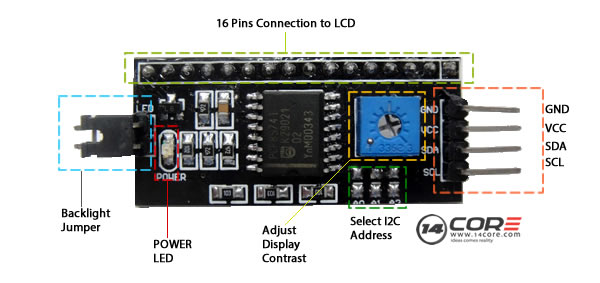
\includegraphics[width=12cm]{I2C-PCF8574-LCD-ADAPTER}
  \caption{I2C-adapter for an LCD display LCM1602-I2C based on the PCF8574 I/O
    expander.}
  \label{fig:i2c-pcf8574-lcd-adapter}
\end{figure}

There are lots of device examples that can be connected to a micro-controller
through an \gls{I2C} bus.  One of such devices is the I/O ports expander
PCF8574.  This is a special chip that allows us to set and read digital values
from its 8 digital pins through I2C bus and thus providing a way to control up
to 8 digital devices.  In other words, PCF8574 is a eight-channel I/O expander.

There is a special adapter based on PCF8574 (see
fig. \ref{fig:i2c-pcf8574-lcd-adapter}) for connecting a liquid-crystal display
(LCD) to a micro-controller through the I2C bus.  Many of such LCDs have
pre-soldered I2C module on them, or it is possible to buy such module separately
for soldering.  Some LCD models have an embedded I2C interface and don't require
a special I2C adapter at all, as all the required circuitry is already present
on the LCD board.

In this section we are going to use the same I/O port expander as is shown on
fig. \ref{fig:i2c-pcf8574-lcd-adapter} to blink LEDs and thus to understand the
I2C bus.  Although there is an Arduino library for working with
PCF8574\footnote{\url{https://www.arduino.cc/reference/en/libraries/pcf8574/}},
we will be using only the
``Wire''\footnote{\url{https://www.arduino.cc/reference/en/language/functions/communication/wire/}}
library that is embedded in Arduino IDE.

It should be noted that the PCF8574 module (see
fig. \ref{fig:i2c-pcf8574-lcd-adapter}) has the area with groups of three
contact pads (``A0'', ``A1'' and ``A2'') marked on the figure as ``Select I2C
Address'' -- by adding jumpers between those contacts we can change the I2C
address of the I2C device.  Having three places for jumpers we get $2^3 = 8$
combinations of them, and thus 8 possible addresses.

\tableLCM{en}

In the table \ref{table:i2c-lcm1602-addressing} all the possible combinations of
the jumpers and respective I2C addresses of the module are
shown.\footnote{Source:
\url{https://static.chipdip.ru/lib/807/DOC015807788.pdf}}

As we discussed above, in fact eight bits are used to encode the I2C device
address, where the seven upper bits (\texttt{A6-A0}) encode the address itself,
and the lower bit encodes the direction of data transmission -- either from the
controller to a target or vice versa.  Changing the values on A0-A2 pins (the
first three rows in the table \ref{table:i2c-lcm1602-addressing}) change the
device address: $V_{DD}$ means the voltage of power supply and $V_{SS}$ means
the ground.  Bits from A3 through A6 have fixed values.

\begin{figure}[H]
  \centering
  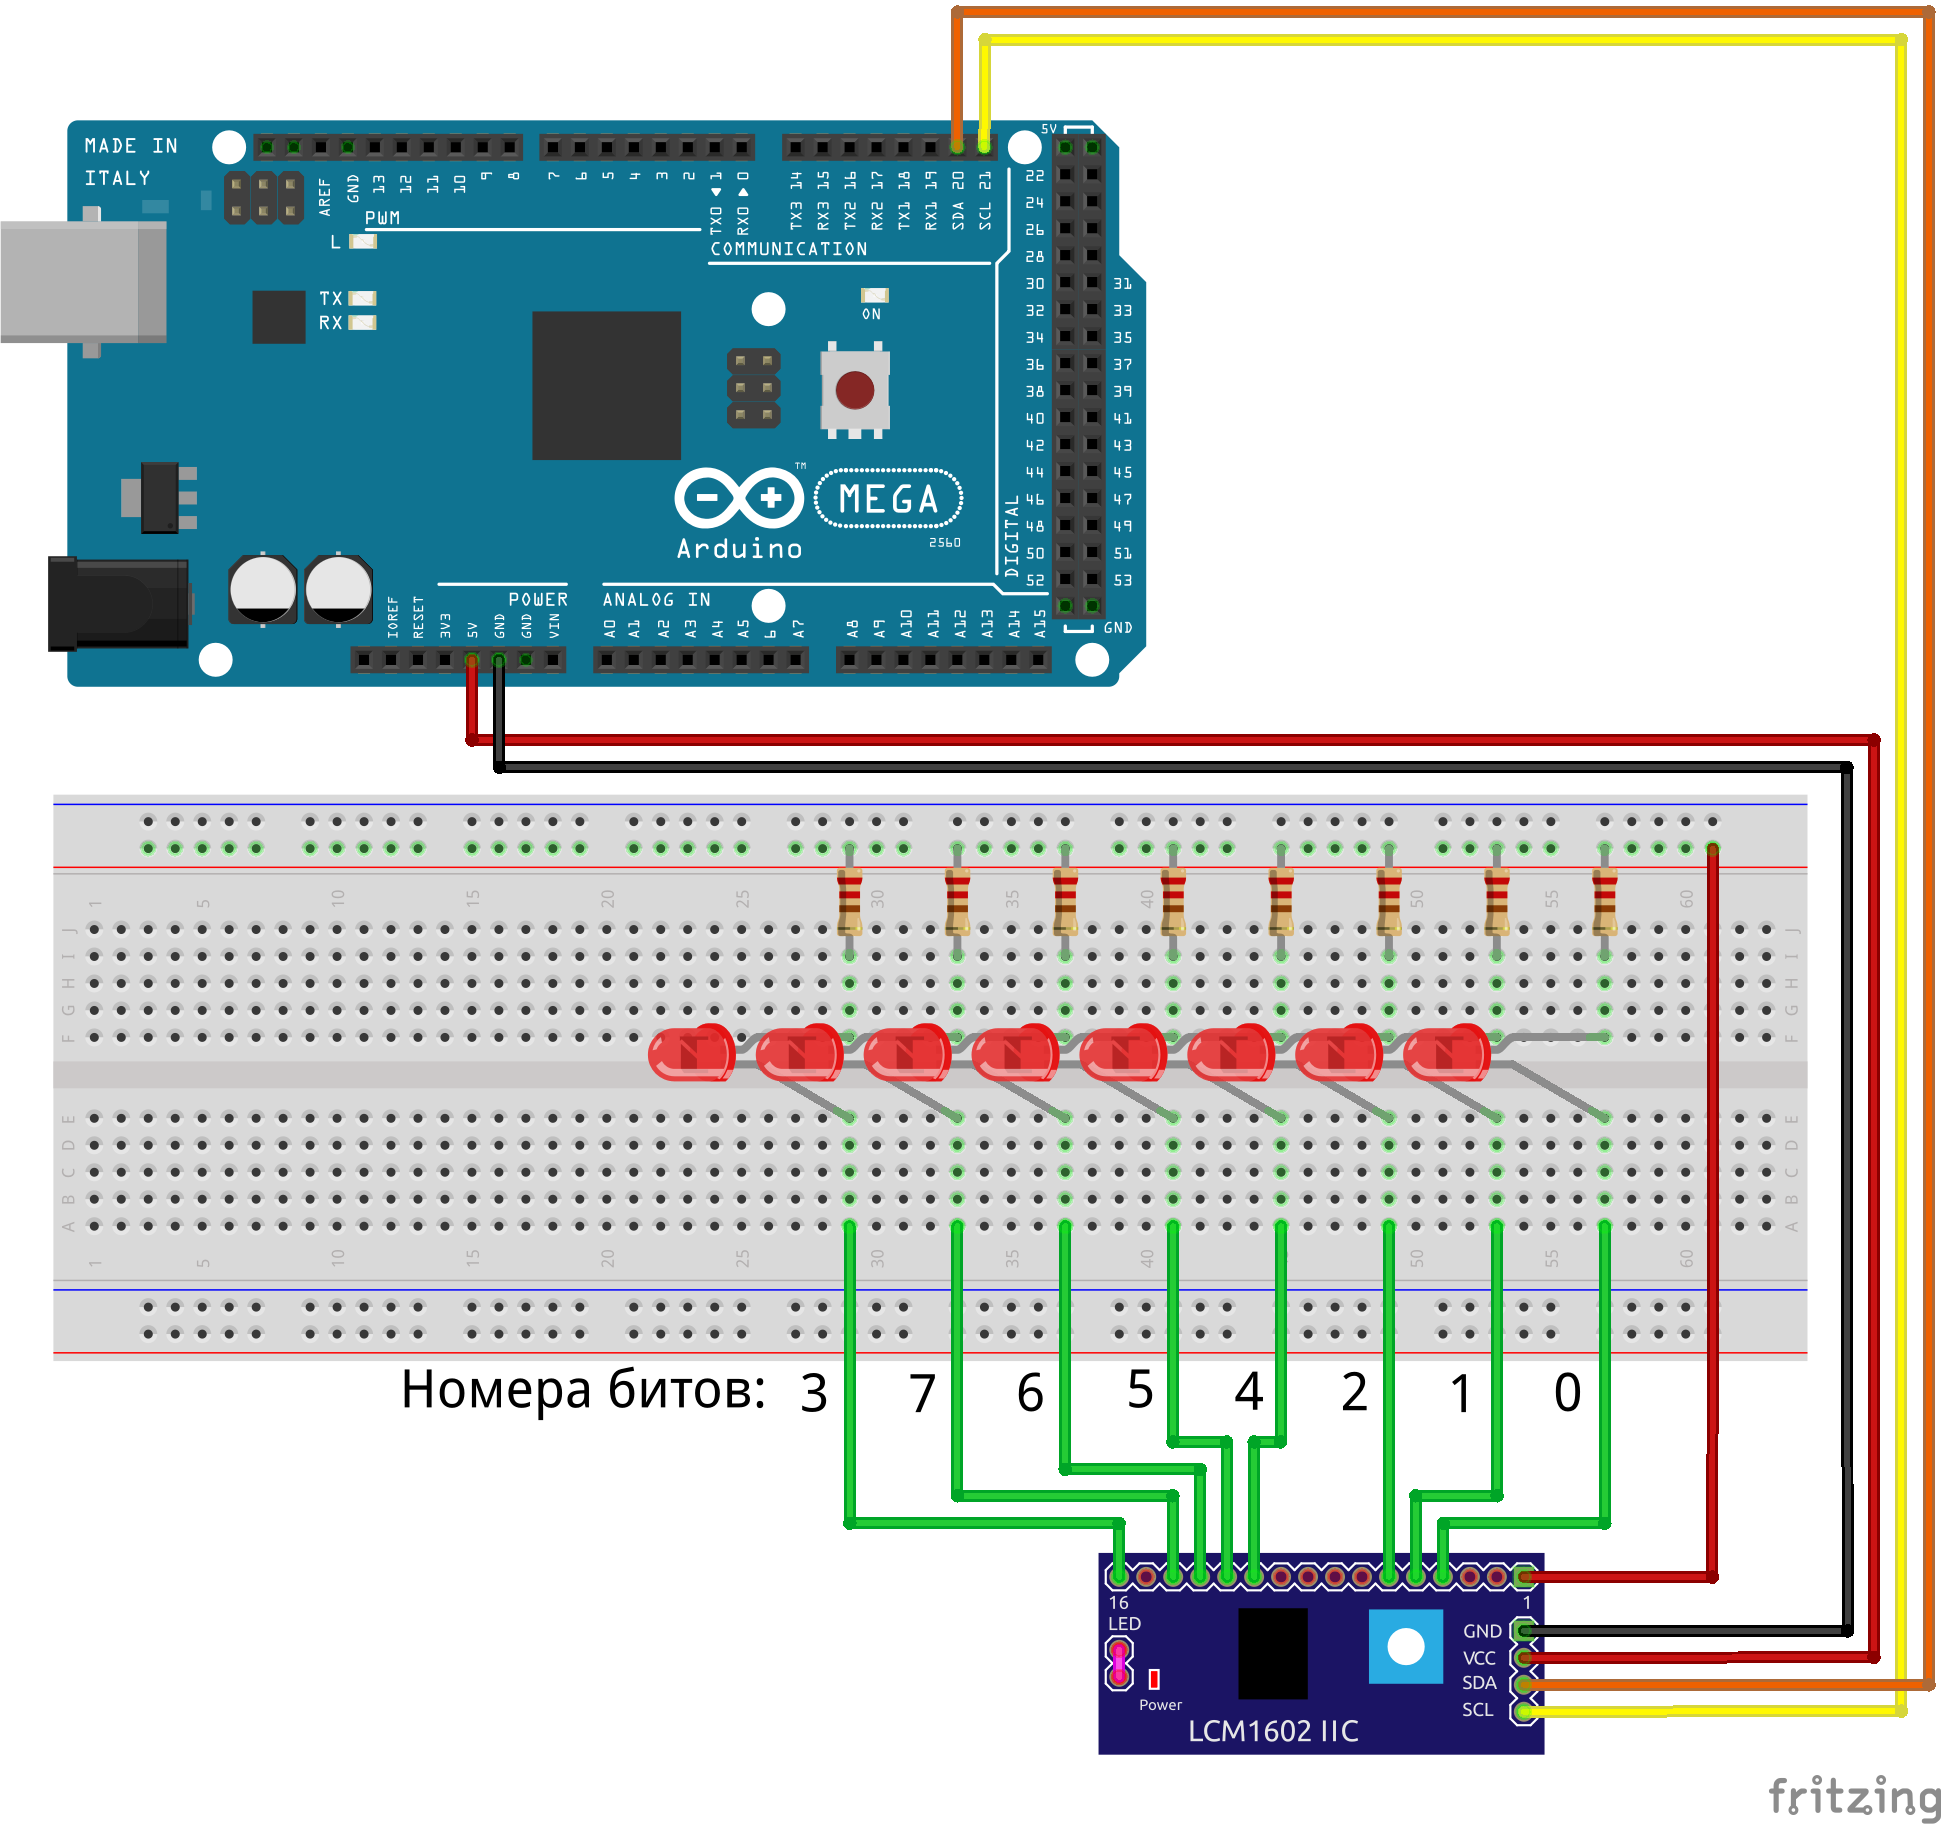
\includegraphics[width=12cm]{schematics/lcm1602-i2c-leds}
  \caption{LCM1602 I2C module based on PCF8574 chip with eight connected LEDs.}
  \label{fig:lcm1602-i2c-leds}
\end{figure}

Let's use the same module as is shown on the fig.
\ref{fig:i2c-pcf8574-lcd-adapter} for our project and connect one LED to each of
the eight I/O pins of the module.  Bits that we write into the module will
directly affect the state of LEDs.  On fig. \ref{fig:lcm1602-i2c-leds} one of
the possible variants of the circuit for the project is shown.  All the
resistors are rated at 220 Ohm.

It should be noted that all the LED anodes on the schematics
\ref{fig:lcm1602-i2c-leds} are connected through resistors to the 5V bus and the
cathodes are connected to the I2C module, which means that the LEDs control is
inverted.  The reason for this is that pulling down is more effective for
controlling LEDs.  When the I2C module pulls an LED cathode down to the ground
then current flows from 5V through the resistor, then through the LED and the
I2C module to the ground.  This configuration is recommended by the manufacturer
of the chip.\footnote{\url{https://static.chipdip.ru/lib/205/DOC000205430.pdf}}

\end{document}
